% Para iniciar una sección debe escribirse
%\section{Nombre de la sección}
% Lo anterior inmediatamente creará la sección y la numerará.

\section*{Objetivos}
\subsection*{Generales}
\begin{itemize}
    \item Introducir a los alumnos a la práctica de ensamblado de circuitos digitales
\end{itemize}

\subsection*{Específicos}
\begin{itemize}
    \item Demostrar la necesidad de mantener un estado estable de entrada (pull-up/pull-down)
    \item Acondicionar los circuitos para mantener un voltaje de operación óptimo
    \item Mostrar las operaciones lógicas básicas en funcionamiento en un circuito implementado físicamente
    \item Contrastar los diseños teóricos con los resultados experimentales de los circuitos implementados físicamente
\end{itemize}

\section{Introducción}
\subsection{Niveles lógicos}
\label{subsection:NivelesLogicos}
Cuando se trabaja con lógica digital la representación de un estado se hace utilizando lógica binaria, la cuál requiere
de dos estados claramente definidos: $1$ y $0$.

A nivel físico, dichos estados pueden a su vez representarse con distintos tipos de magnitudes medibles, tales como 
un voltaje constante, una corriente, una temperatura, o un valor de luminosidad.

Asimismo, tal y como se ha explicado en clase, dependiendo de la tecnología utilizada (TTL, CMOS, LVCMOS, etc) los niveles
lógicos se representan con un nivel de voltaje que obedece a los umbrales de la Tabla \ref{Table:umbralesLogicos}:

\begin{table}[H]
    \centering
    \begin{tabular}{|c|c|c|}
        \hline
        \textbf{Estado} & \textbf{CMOS} & \textbf{TTL}  \\ \hline
        \textbf{0}      & 0.0 V - 1.5 V & 0.0 V - 0.8 V \\ \hline
        \textbf{1}      & 3.5 V - 5.0 V & 2.0 V - 5.0 V \\ \hline
    \end{tabular}
    \caption{Umbrales de voltaje para niveles lógicos}
    \label{Table:umbralesLogicos}
\end{table}

\subsection{Implementación experimental de circuitos de lógica digital}
Para que los diseños que se describen matemáticamente puedan implementarse es necesario hacer uso de dispositivos capaces
de trabajar con la representación de niveles a través de magnitudes físicas. Estos dispositivos pueden ser desde algo tan 
básico como trabajar directamente a nivel de transistores o incluso la implementación de sistemas complejos de electrónica digital
a través de lenguajes de descripción por hardware en dispositivos FPGA o SoC/MPSoC.

En este laboratorio se hará uso de la tecnología más utilizada en la década de los 80's: 
\textbf{Compuertas Lógicas con Circuitos Integrados}. Dependiendo de disponibilidad en las tiendas, estos circuitos integrados
pueden ser de tecnología TTL o CMOS. Los circuitos Integrados (\textbf{CI}) que implementan compuertas lógicas permiten al diseñador
desentenderse de lidiar con la configuración de los transistores para que éstos trabajen en la región adecuada (corte/saturación)
y tienen un costo relativamente bajo. Es por estas razones que son la metodología preferia a nivel de academia para introducir a
los estudiantes al esta nueva área de conocimiento.

Normalmente los circuitos integrados poseen más de una compuerta lógica en cada empaquetado, lo que permite optimizar la cantidad de
componentes que requiere un diseño final. En la Figura \ref{Fig:CompuertasEnCI} se muestra el diagrama de un Circuito Integrado de
Compuertas NOT: la alimentación al circuito integrado es vital para que funcione (pines \textit{Vcc} y \textit{GND})

\begin{figure}[H]
    \centering
    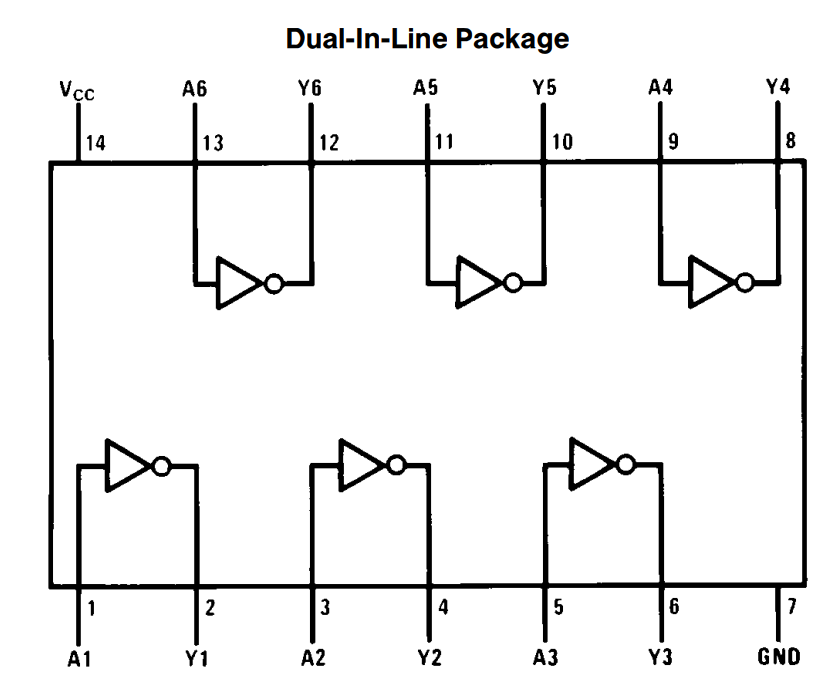
\includegraphics[scale=0.3]{images/7404.PNG}
    \caption{Compuertas dentro de un Circuito Integrado}
    \label{Fig:CompuertasEnCI}
\end{figure}

Los circuitos integrados tienen un código único base que indica la funcionalidad que realizan. A continuación se muestran algunos ejemplos
\footnote{Listado completo de códigos:
\url{https://en.wikibooks.org/wiki/Digital_Circuits/7400_Series}}:

\begin{itemize}
    \item Compuerta AND de 2 entradas $->$ \textbf{74xx08}
    \item Compuerta OR de 2 entradas $->$ \textbf{74xx32}
    \item Compuerta XOR de 2 entradas $->$ \textbf{74xx86}
    \item Compuerta NOR de 2 entradas $->$ \textbf{74xx02}
    \item Compuerta NAND de 2 entradas $->$ \textbf{74xx00}
    \item Compuerta NOT $->$ \textbf{74xx04}
\end{itemize}

Es importante resaltar que las letras \textbf{xx} en el código de cada circuito integrado determinan la tecnología a la que pertenece
la familia de circuitos integrados. Por ejemplo, los más uitlizados en nuestro país son:
\begin{itemize}
    \item Tecnología TTL  $->$ \textbf{LS}
    \item Tecnología CMOS $->$ \textbf{HC}
\end{itemize}

\vspace{20pt}
A continuación unos ejemplos de circuitos integrados comerciales:

\begin{itemize}
    \item \textbf{74HC08}: CI con 4 compuertas AND de tecnología CMOS
    \item \textbf{74LS04}: CI con 6 compuertas NOT de tecnología TTL
    \item \textbf{74HC32}: CI con 4 compuertas OR de tecnología CMOS
\end{itemize}


\subsection{Niveles lógicos en Entradas/Salidas}
Como se constató en la sección \ref{subsection:NivelesLogicos}, es de vital importancia la constancia de una magnitud física que represente un nivel lógico.
En otras palabras: si se desea representar un $0$ utilizando tecnología TTL, lo ideal es que el voltaje correspondiente a ese estado sea 0.0V; sin embargo, esto
es algo casi imposible a nivel experimental, por lo que un voltaje entre 0.0V y 0.8V bastará para representar dicho valor.

Cuando los circuitos integrados están correctamente alimentados (voltaje y corriente de alimentación estables), éstos se encargan de mantener los niveles (umbrales) de voltaje de \textbf{salida} en el rango adecuado para representar
cualquiera de los dos estados lógicos posibles. Las \textbf{entradas} a los CI deben estar también en los rangos (umbrales) adecuados para funcionamiento, algo que es responsabilidad completa del diseñador cuidar.

Por esta razón, cuando la entrada de un circuito integrado no está siendo manejada por la salida de otro circuito integrado es necesario cuidar que los niveles de voltaje estén siempre dentro de los umbrales.

Si es un usuario que interactúa con dichas entradas a través de pulsadores o interruptores, cuando éstos se encuentran \emph{abiertos} (desconectados), el voltaje en la entrada cambia a un valor incierto (ni 1, ni 0)
de forma aleatoria. En la Figura \ref{Fig:NoPull} se muestran los casos posibles de este problema.

\begin{figure}[H]
    \centering
    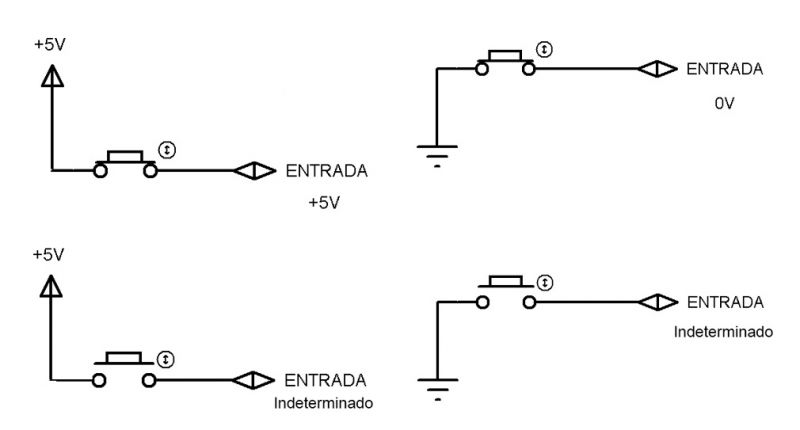
\includegraphics[scale=0.5]{images/noPull.jpg}
    \caption{Valores inciertos de entrada al desconectar el interruptor}
    \label{Fig:NoPull}
\end{figure}


\subsection{Resistencias \emph{pull-up} y \emph{pull-down}}
Para mitigar el problema de entradas inciertas se colocan resistencias que mantendrán un nivel de voltaje, ya sea en alto (resistencias \emph{pull-up}) o en bajo (resistencias \emph{pull-down}) mientras el pulsador
o interruptor se encuentra desconectado. Cuando el usuario activa el interruptor, la resistencia \emph{pull-up} o \emph{pull-down} tiene una impedancia muy alta comparado con la resistencia interna del mismo interruptor, por lo
que la resistencia equivalente combinada del circuito de entrada es prácticamente la resistencia interna del interruptor (tiende a ser 0). Esto permite cambiar de estados (entre 1 y 0) rápidamente sin permanecer por mucho
tiempo fuera de cualquier umbral que cause un estado indeseado a la salida. En las Figuras \ref{Fig:PullDown} y \ref{Fig:PullUp} se muestra el diagrama para la correcta conexión en los circuitos de entrada.

\begin{figure}[H]
    \centering
    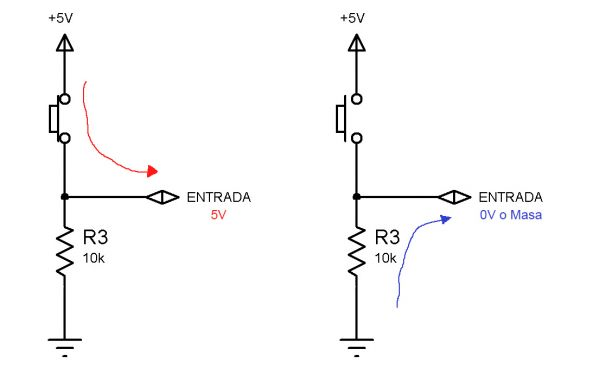
\includegraphics[scale=0.5]{images/pullDown.jpg}
    \caption{Entrada con Resistencias \emph{Pull-Down}}
    \label{Fig:PullDown}
\end{figure}

\begin{figure}[H]
    \centering
    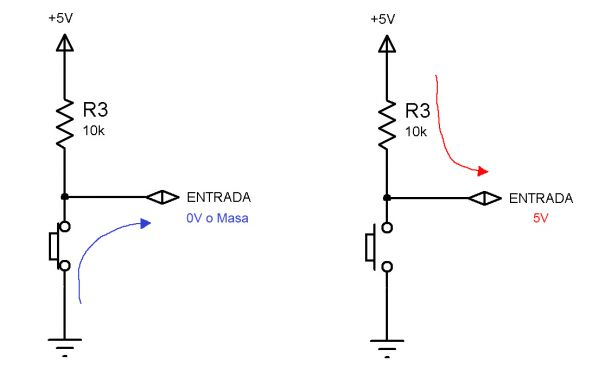
\includegraphics[scale=0.5]{images/pullUp.jpg}
    \caption{Entrada con Resistencias \emph{Pull-Up}}
    \label{Fig:PullUp}
\end{figure}

Normalmente se requiere que las resistencias utilizadas para \emph{pull-up} o \emph{pull-down} no tengan un valor muy alto, de lo contrario sería el equivalente a mantener el circuito abierto,
lo que conllevaría a un estado incierto. Sin embargo, una resistencia muy pequeña causaría un corto-circuito cuando se presiona el pulsador. Cabe resaltar que estas resistencias causan un aumento leve
en el consumo de corriente estática del circuito, por lo que en aplicaciones que requieran maximizar la vida de la batería el análisis del valor óptimo debe realizarse con cautela.

Sin embargo, para usos prácticos de laboratorio, las resistencias pueden tener un valor entre $1k\ohm$ y $10k\ohm$.

\subsubsection{¿\emph{Pull-Up} o \emph{Pull-Down}? ¿Cuál uso entonces?}
Depende de la aplicación. Una resistencia \emph{pull-down} mantiene el estado por defecto en \textbf{0}; mientras una resistencia \emph{pull-up} mantiene el estado por defecto en \textbf{1}.
Hay aplicaciones de elecrónica digital que utilizan la llamada \emph{lógica negada} y es donde comúnmente se utilizan \emph{pull-up}.

En general durante las prácticas de este laboratorio se utilizarán resistencias en configuración \textbf{\emph{pull-down}}.


\subsection{Alimentación de Circuitos Integrados}
Como se ha mencionado con anterioridad, la alimentación estable a los circuitos integrados es fundamental para el correcto funcionamiento de los mismos, y por ende, del proyecto completo.

Las compuertas lógicas que se utilizarán durante todas las prácticas utilizan una alimentación de 5.0 Volts.

Para lograr esto hay varias alternativas que pueden tomarse:
\begin{itemize}
    \item Alimentación directa por USB (de una batería portable, por ejemplo)
    \item Una batería Li-Po de 3.7V con un \emph{step-up converter} y un regulador lineal de 5V
    \item Una batería de 9V con un regulador lineal de 5V
    \item Un conjunto de 3 baterías alcalinas de 1.5V (AA, AAA) en serie
    \item Un conjunto de 4 baterías recargables de 1.2V (AA, AAA) en serie
    \item Un cargador de teléfono \textbf{de buena calidad} capaz de proveer una salida de voltaje constante
    \item Una fuente de computadora de escritorio que ya no esté en uso
\end{itemize}

\vspace{20pt}

Un regulador lineal puede ser cualquiera de los siguientes circuitos integrados:
\begin{itemize}
    \item MAX603
    \item LM1084
    \item 7805
\end{itemize}

\pagebreak

\section{Desarrollo Experimental}
\subsection{Materiales y Equipo}

Cada grupo debe llevar su material y equipo de trabajo durante las prácticas. Pregunte a su profesor qué \emph{Equipo de Laboratorio} puede ser prestado
de parte del laboratorio de instrumentación. El laboratorio de instrumentación no tiene disponibilidad de ningún elemento de la lista \emph{Materiales}.

\subsubsection*{Materiales}
\begin{itemize}
    \item 1x dip-switch de 4 posiciones (o más)
    \item 4x pulsadores (si no consiguiesen el dip-switch de 4 posiciones)
    \item 1x fuente de alimentación (ver apartado anterior con todas las alternativas)
    \item 2x capacitores electrolíticos de 47 $\mu$F 16V
    \item 2x capacitores cerámicos de 100nF 25V
    \item 4x resistencias de 10 k$\ohm$
    \item 4x resistencias de 1 k$\ohm$
    \item 4x LED de cualquier color (excepto infrarrojo o ultravioleta)
    \item 6x metros de alambre para protoboard calibre 22. Compren al menos 2 colores para los 6 metros. \textbf{No usen \emph{UTP}}, aunque eso les quieran vender.
    \item 2x 74xx08 (AND)
    \item 2x 74xx04 (NOT)
    \item 2x 74xx32 (OR)
\end{itemize}


\subsubsection*{Equipo de Laboratorio}
\begin{itemize}
    \item 1x Pinzas delgadas
    \item 1x Cortaalambres
    \item 1x Pelador de alambres para calibre 22 (opcional)
    \item 1x Tijeras pequeñas o cortauñas (si no tienen pela alambres)
    \item 1x Protoboard de al menos 2 galletas (puede juntar 2 protoboards de 1 galleta)
    \item 1x Multímetro digital para medir voltaje
\end{itemize}

\subsection{Procedimiento}
\subsubsection{Fuente de alimentación}
Pregunte a su instructor cómo construir una fuente con los insumos que tiene disponibles.

\subsubsection{Primer circuito con Electrónica Digital}
Implementar un circuito simple para demostrar uno de los \emph{Teoremas de De Morgan} utilizando las compuertas disponibles.
Solamente utilice dos entradas con el dip-switch para hacer la demostración.
Utilice un LED como salida de cada operación, limitando su corriente con una resistencia de 1k$\ohm$.

\vspace{14pt}

Debe realizar dos operaciones. Por ejemplo, si se decide demostrar el teorema de la Ecuación \ref{Eq:DeMorgan1}.

\begin{equation}
    \overline{A B} = \bar{A} + \bar{B}
    \label{Eq:DeMorgan1}
\end{equation}

Se debe implementar el circuito $\overline{A B}$ y por aparte también deberá ensamblar el circuito $\bar{A} + \bar{B}$, utilizando las mismas dos entradas en paralelo.
Cada circuito deberá tener una salida independiente visible con un LED.

\subsubsection{Función booleana y reducción con Karnaugh}
De los integrantes de su grupo, busque la persona con el número carnet más bajo: tome los últimos 4 dígitos (no repetidos) de este número.

\vspace{14pt}

Por ejemplo, si el carnet es \textbf{200815521} los últimos 4 dígitos no repetidos son: \textbf{1}, \textbf{2}, \textbf{5} y \textbf{8}.

\vspace{14pt}

Ahora construya una función booleana utilizando la sumatoria de los dígitos obtenidos. Tomando el ejemplo anterior, sería:

$$ f = \sum{1,2,5,8} $$

Codifique los dígitos en BCD y asigne el bit menos significativo a el dip-switch localizado físicamente más a la derecha en el protoboard 
(pregunte a su instructor si quedan dudas).

\vspace{14pt}

Finalmente, reduzca la función utilizando un Mapa de Karnaugh para simplificar los mintérminos obtenidos e implemente el circuito, usando como entrada 
el dip-switch con resistencias \emph{pull-down} y la salida con un LED con limitación de corriente.

